
During August 2022 a testbeam took place in Santa Chiara hospital in Pisa, where a new accelerator designed for both medical research and R$\&$D in FLASH-RT, and for this reason called "ElectronFlash", have been installed a few months ago. 

The motivation of the testbeam measurements were testing TJ-Mopopix1 in condition different from the one forseen during the design and also testing the mechanical and the DAQ setup for other future measurement. TJ-Monopix1 is supposed to be employed for tracking in HEP experiments while our goal was testing the possibility of integrating the charge released by more particles at ultra high hit rate achievable with the accelerator.
\red{Una frase di disclaimer sul fatto che non siamo riusciti a testare quello che volevamo.}

In medical physics the dose is indeed the standard parameter to charaterize the beam beacause of its obvious relation with the damage caused in the patient: firstly the oncologists prescribe a certain dose taking into account the efficacy of the treatment and then the medical physicists, on the basis of simulations, decide the energy and the intensity of the beams to dispense the prescribed dose amount.
By the point of view of the instrumentation and the testing on it, a more common and usefull parameter is instead the rate or the fluence of particles.  
The conversion between the two quantity can be find thinking to the definition of dose: it is the concentration of energy deposited in tissue as a result of an exposure to ionizing radiation. 
Assuming total absorption of electrons in water, defined by law as the ordinarily reference medium, the dose can be expressed as: 
\begin{equation}
   D[Gy] = \frac{N E[eV]}{\rho[g/cm^3] A[cm^2] x[cm]}
\end{equation}
After having applyed the conversion of the energy from \si{eV} to \si{J} and noticed that E/$\rho$x roughly corresponds to the stopping power S of electrons in water, a simple estimation of the dose released in water is:
\begin{equation}
   D[Gy] = 1.602\;10^{-10}\,N[cm^{-2}]\,S[MeV cm^2/g]
\end{equation}


\section{Apparatus description}
   The accelerator is placed in a bunker inside the hospital: to shield the outdoor from ionizing radiation the bunker has very thick walls of cementum and both the control units of the accelerator and of the detector were placed outside the bunker. 
   For practicability reasons the power supply were the only device to be placed inside the bunker. 
   \subsection{Accelerator}
      \begin{figure}
         \centering
         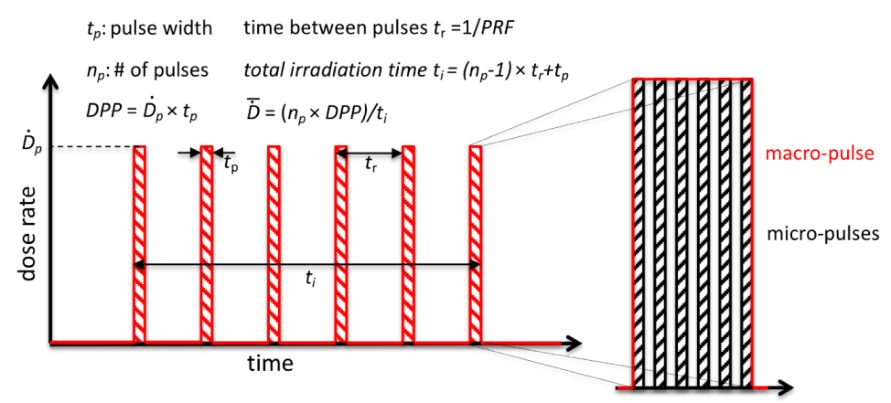
\includegraphics[width=.9\linewidth]{figures/test_beam/beam_structure.pdf}
         \caption{Typical beam structure of a beam with the standard characteristic quantity}
         \label{fig:beam_structure}
      \end{figure}
      \begin{table}
         \begin{center}
         \begin{tabular}{| c | c | c |}
         \hline
      $\bar{D}$ & Dose rate (mean dose rate for a multi-pulse delivery) & 0.005-10000 Gy/s\\
      $\Dot{\bar{D}}$ & Intra pulse dose rate (dose rate in a single pulse) &  0.01-1 10$^6$ Gy/s  \\
      DDP & Dose in a single pulse & 0.04-40 Gy\\
      PRF & Pulse repetition frequency(number of pulses delivered per unit of time) & 1-350 Hz\\
      t$_{p}$ & Pulse width & 0.2-4 \si{\us}\\
      n & Number of pulses & single/pulse train \\
      \hline
         \end{tabular}
         \caption{The parameters that can actually be set by the control unit are the PRF, DDP, t$_p$ and n (in particular singolar irradiation or pulse train), while the other changes consequently.}
         \label{tab:beam_parameters}
         \end{center}
      \end{table}  
      The ElectronFlash accelerator is an electron Linear Accelerator (LINAC) with two energy configurations, at \SI{7}{MeV} and \SI{9}{MeV}, and it can reach ultra high intensity (\SI{40}{Gy/pulse}) keeping the possibility of accessing many different beam parameters and changing them independently from each other. This charateristic is faundamental for research in FLASH-RT, both for the medical aspects and for the studies on detectors; for example is not really clear the dependence of the efficacy of the FLASH effect on the whole dose parameters. ElectronFlash is \red{almost the only one} in the world having this charateristic, \red{ricontrolla sulla review, c'era qualcosa che puoi dire. }    
      The accelerator implements a standard beam structure for RT with electrons (fig. \ref{fig:beam_structure}), that is a macro pulse divided in many micropulses; the parameters used to set the dose and their range of values settable by the control unit is reported in table \ref{tab:beam_parameters}. 

      The accelerator is provided of a set of triod cannons $\sim$\SI{1.2}{m} long and with diameters from \SI{1}{cm} to \SI{12}{cm} and a collimator that can be used as beam shaper to produce a squircle shape.
      The triode, which is made by plexiglass, must be fix to the gun during the irradiation and is needed for producing an uniform dose profile (fig.\ref{fig:dose_profile}) which is desired for medical pourpose via the scattering of electrons with the plexiglass.
      \begin{figure}[h!]
         \centering
         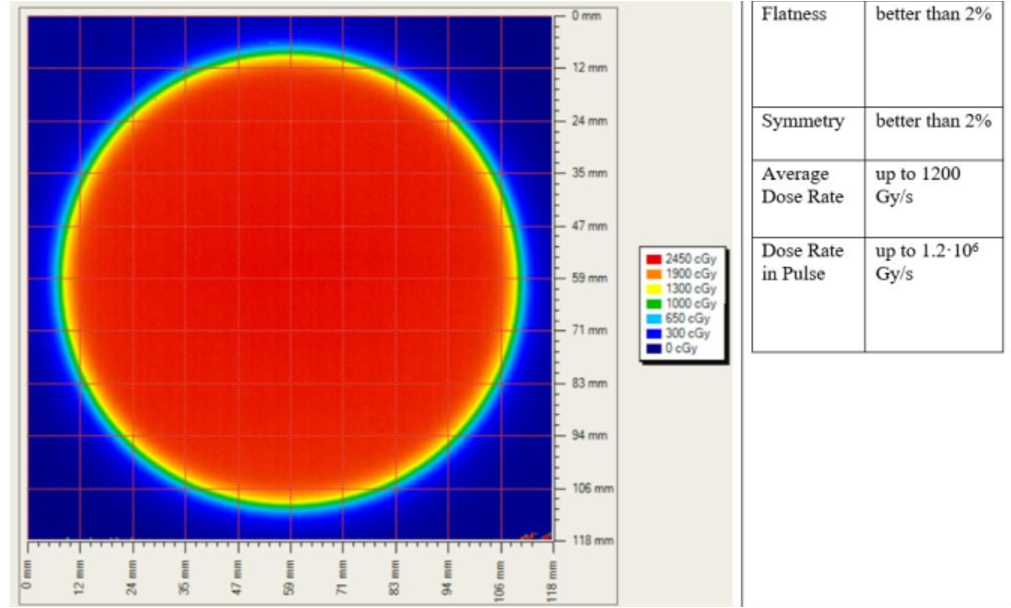
\includegraphics[width=.49\linewidth]{figures/test_beam/dose_profile_10cm.pdf}
         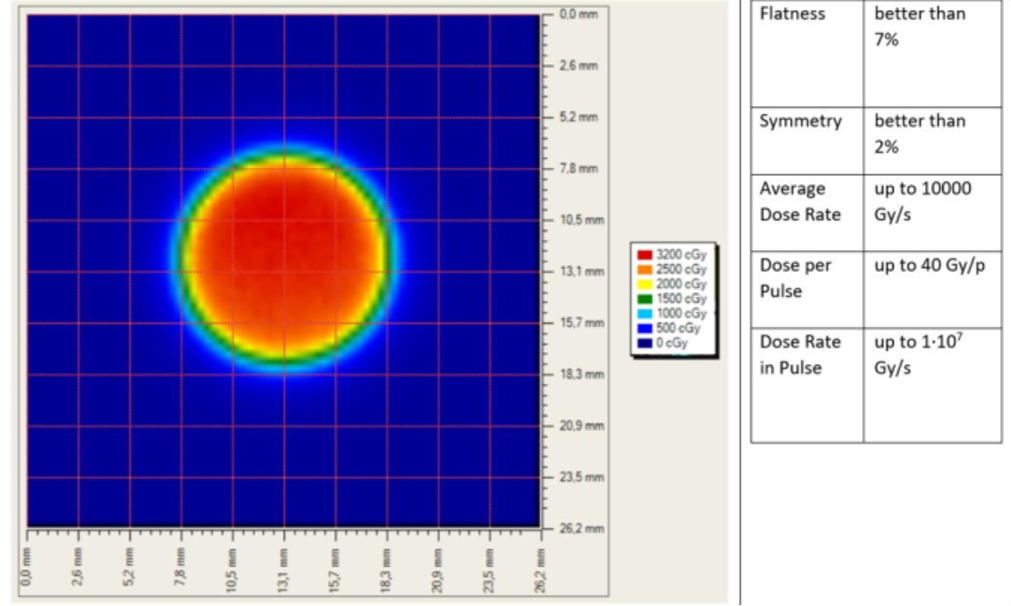
\includegraphics[width=.49\linewidth]{figures/test_beam/dose_profile_1cm.pdf}
         \caption{Two example of x-y isodose curves for two different triodes, \SI{10}{cm} and \SI{1}{cm} respectively, reported by the producer in the manual with the specific of the accelerator (S.I.T. - Sordina IORT Technologies S.p.A.). With the smaller collimator the dose rate in pulse is comparatively higher.}
         \label{fig:dose_profile}
      \end{figure}  

   \subsection{Mechanical carriers}
      The tested detector consists in one chip, the Device Under Test (DUT), mounted on a board and connected to FPGA with same arrangement of figure \ref{fig:}.
      These have been positioned vertically in front of the triode on a table specifically built for the testbeam. The tree board have been enclosed in a box of alluminium with a window on the DUT and with the required holes at the side to enable the biasing via cables and the connection with the DAQ provided via ethernet cable.       
      A trigger signal coming from the control unity and syncronize with the pulses emitted from the beam has been also sent to the FPGA.
      This signal cannot be considered a trigger signal, since being a prototypes TJ-Monopix1 has been designed to be triggerless, but the time of arrival of this signal, which is saved by the FPGA, can allow the reconstruction of the of the arrival of the bunch during the analysis.

      In order to shield the sensor from the whole particles emitted from the gun, two alluminium collimators have been fabricated: one has been positioned at the triode exit while the other in front of the DUT. The collimators are $t$=\SI{32}{mm} thick and have a diameter $d$ equal to \SI{1}{mm}: assuming a beam divergence bigger than $d/t$=1/32 = \SI{1.8}{\degree}, which is the case, the collimator at the triode output was supposed to work as a point source and to reduce the rate on the DUT of a factor at least 4 10${^-4}$. The second one, being near the DUT, was instead supposed to shield the sensor from the electrons which have passed the first one, except for a region of \SI{1}{mm\squared} configurable using \red{come si chiamano quei cacciavitini per settare la posizione?}.  
      \begin{figure}[h!]
         \centering
         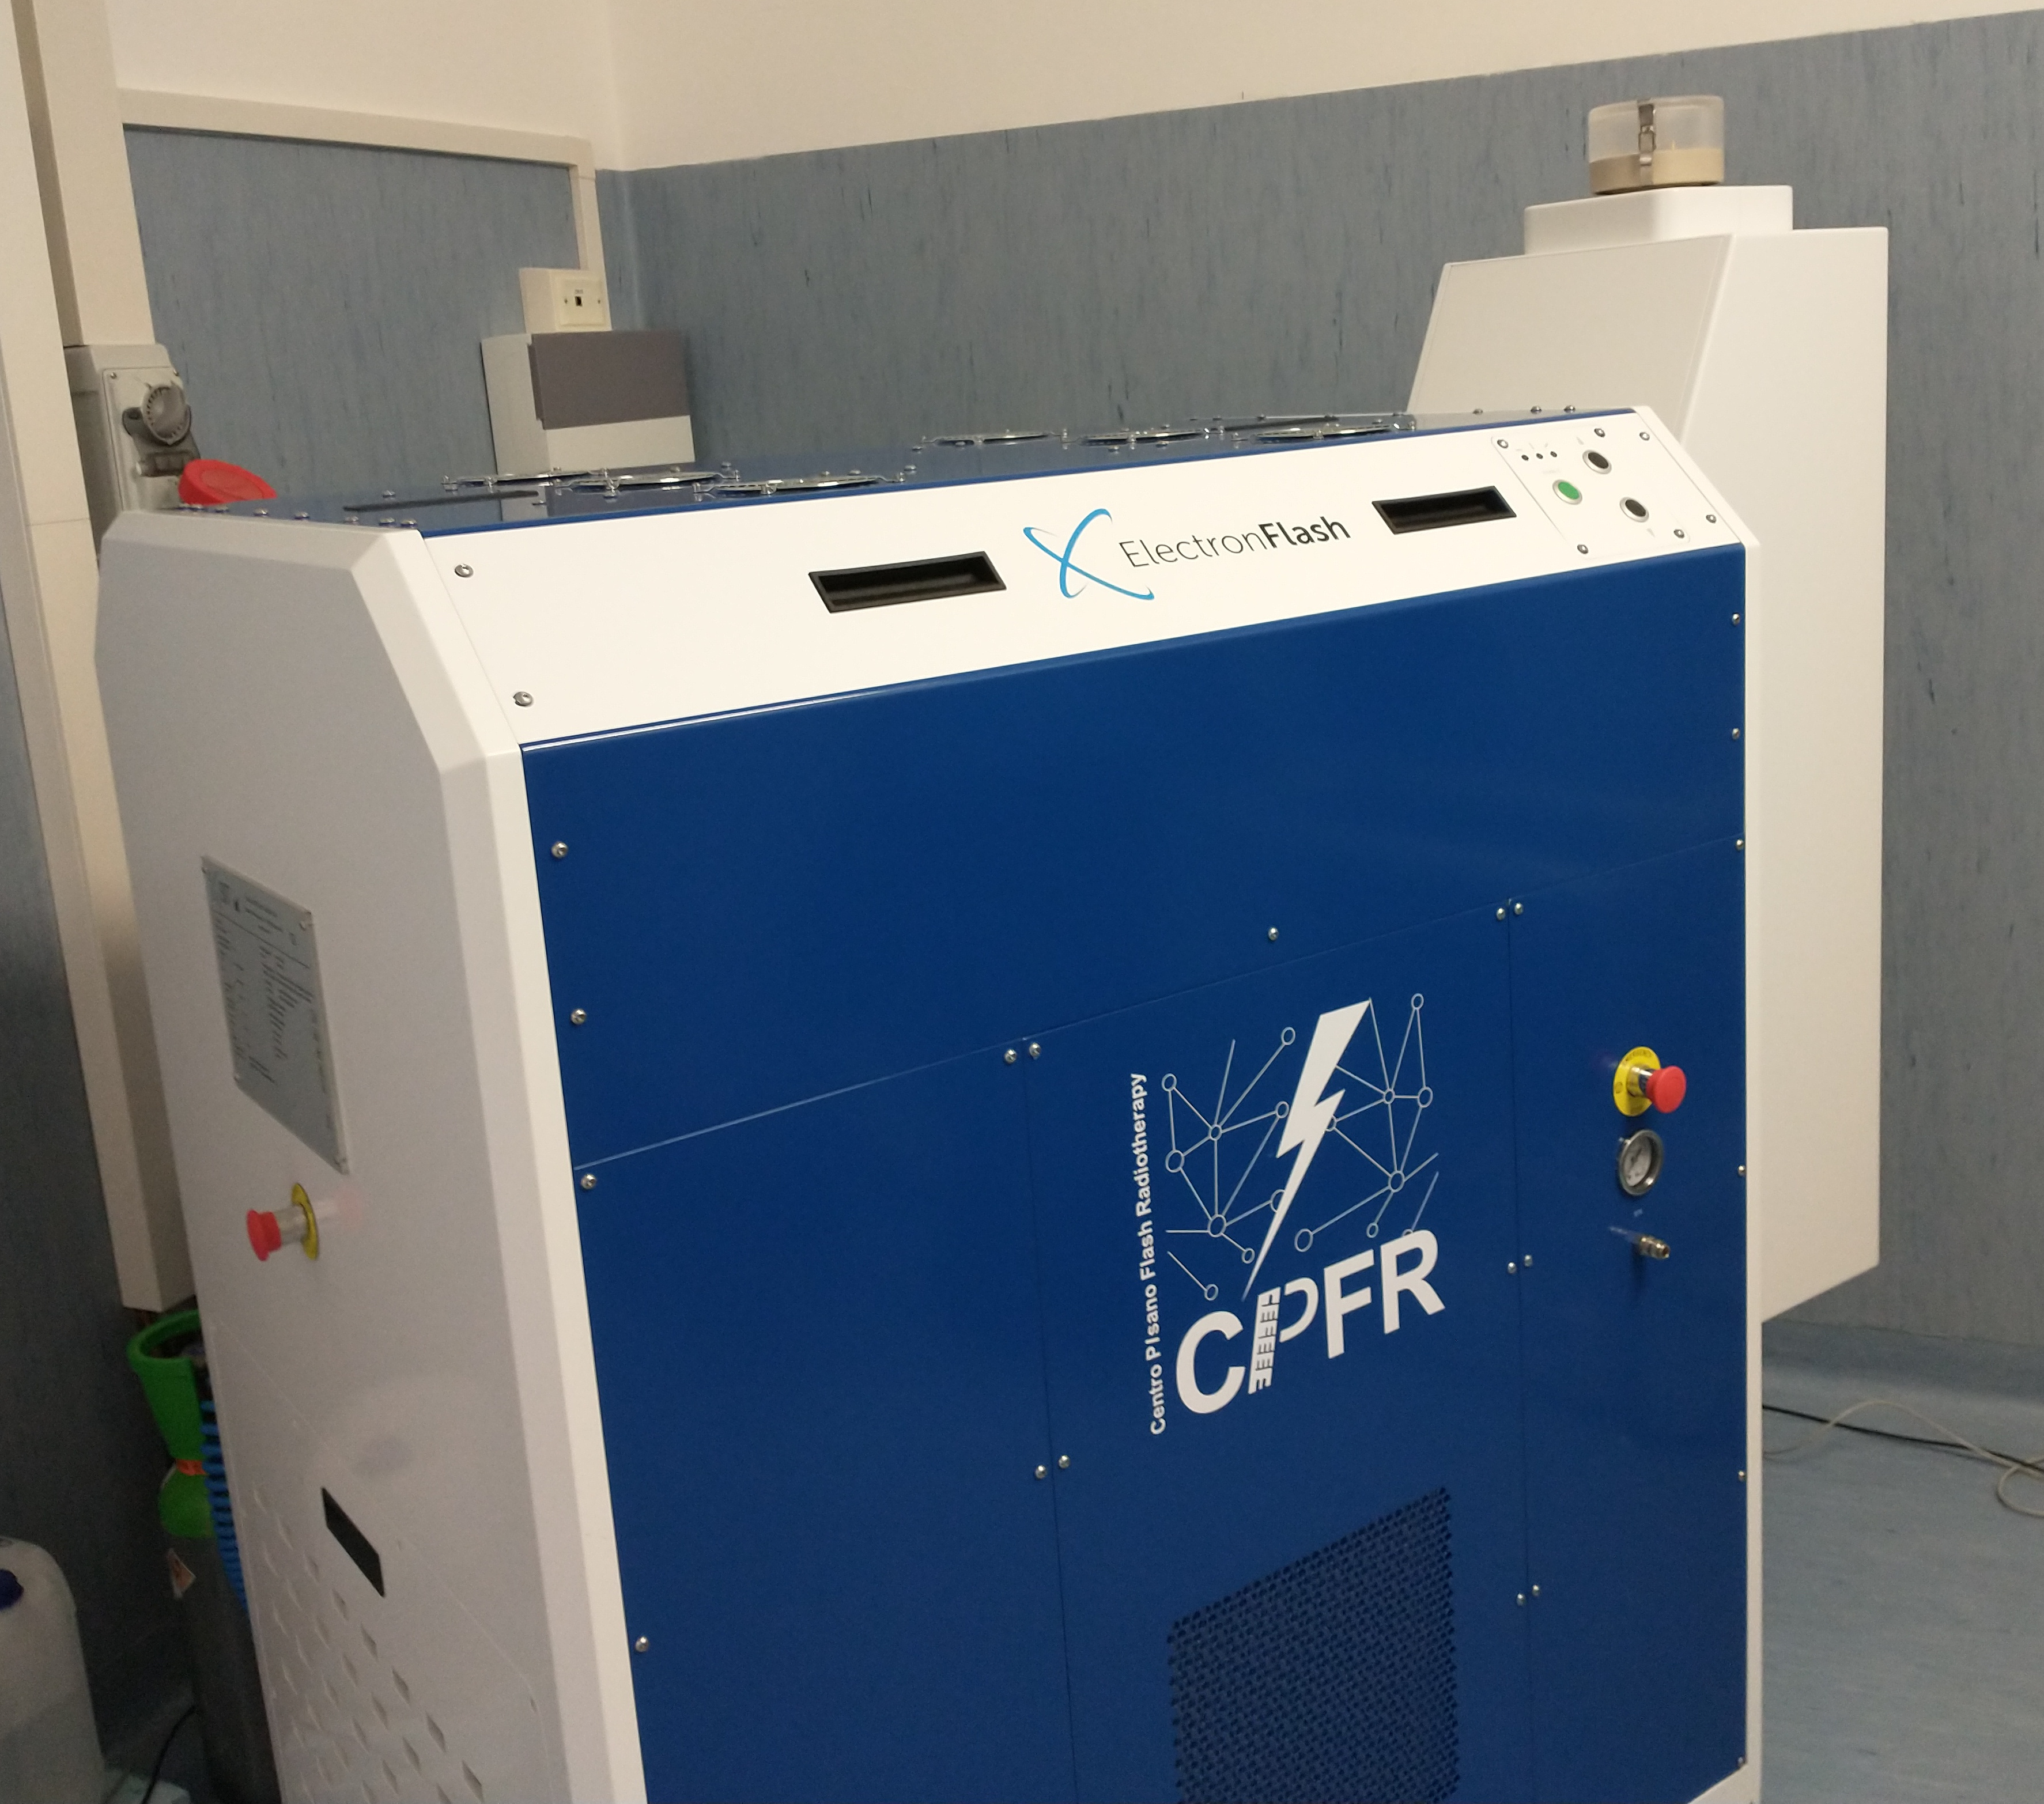
\includegraphics[width=.40\linewidth]{figures/test_beam/electron_flash.jpg}
         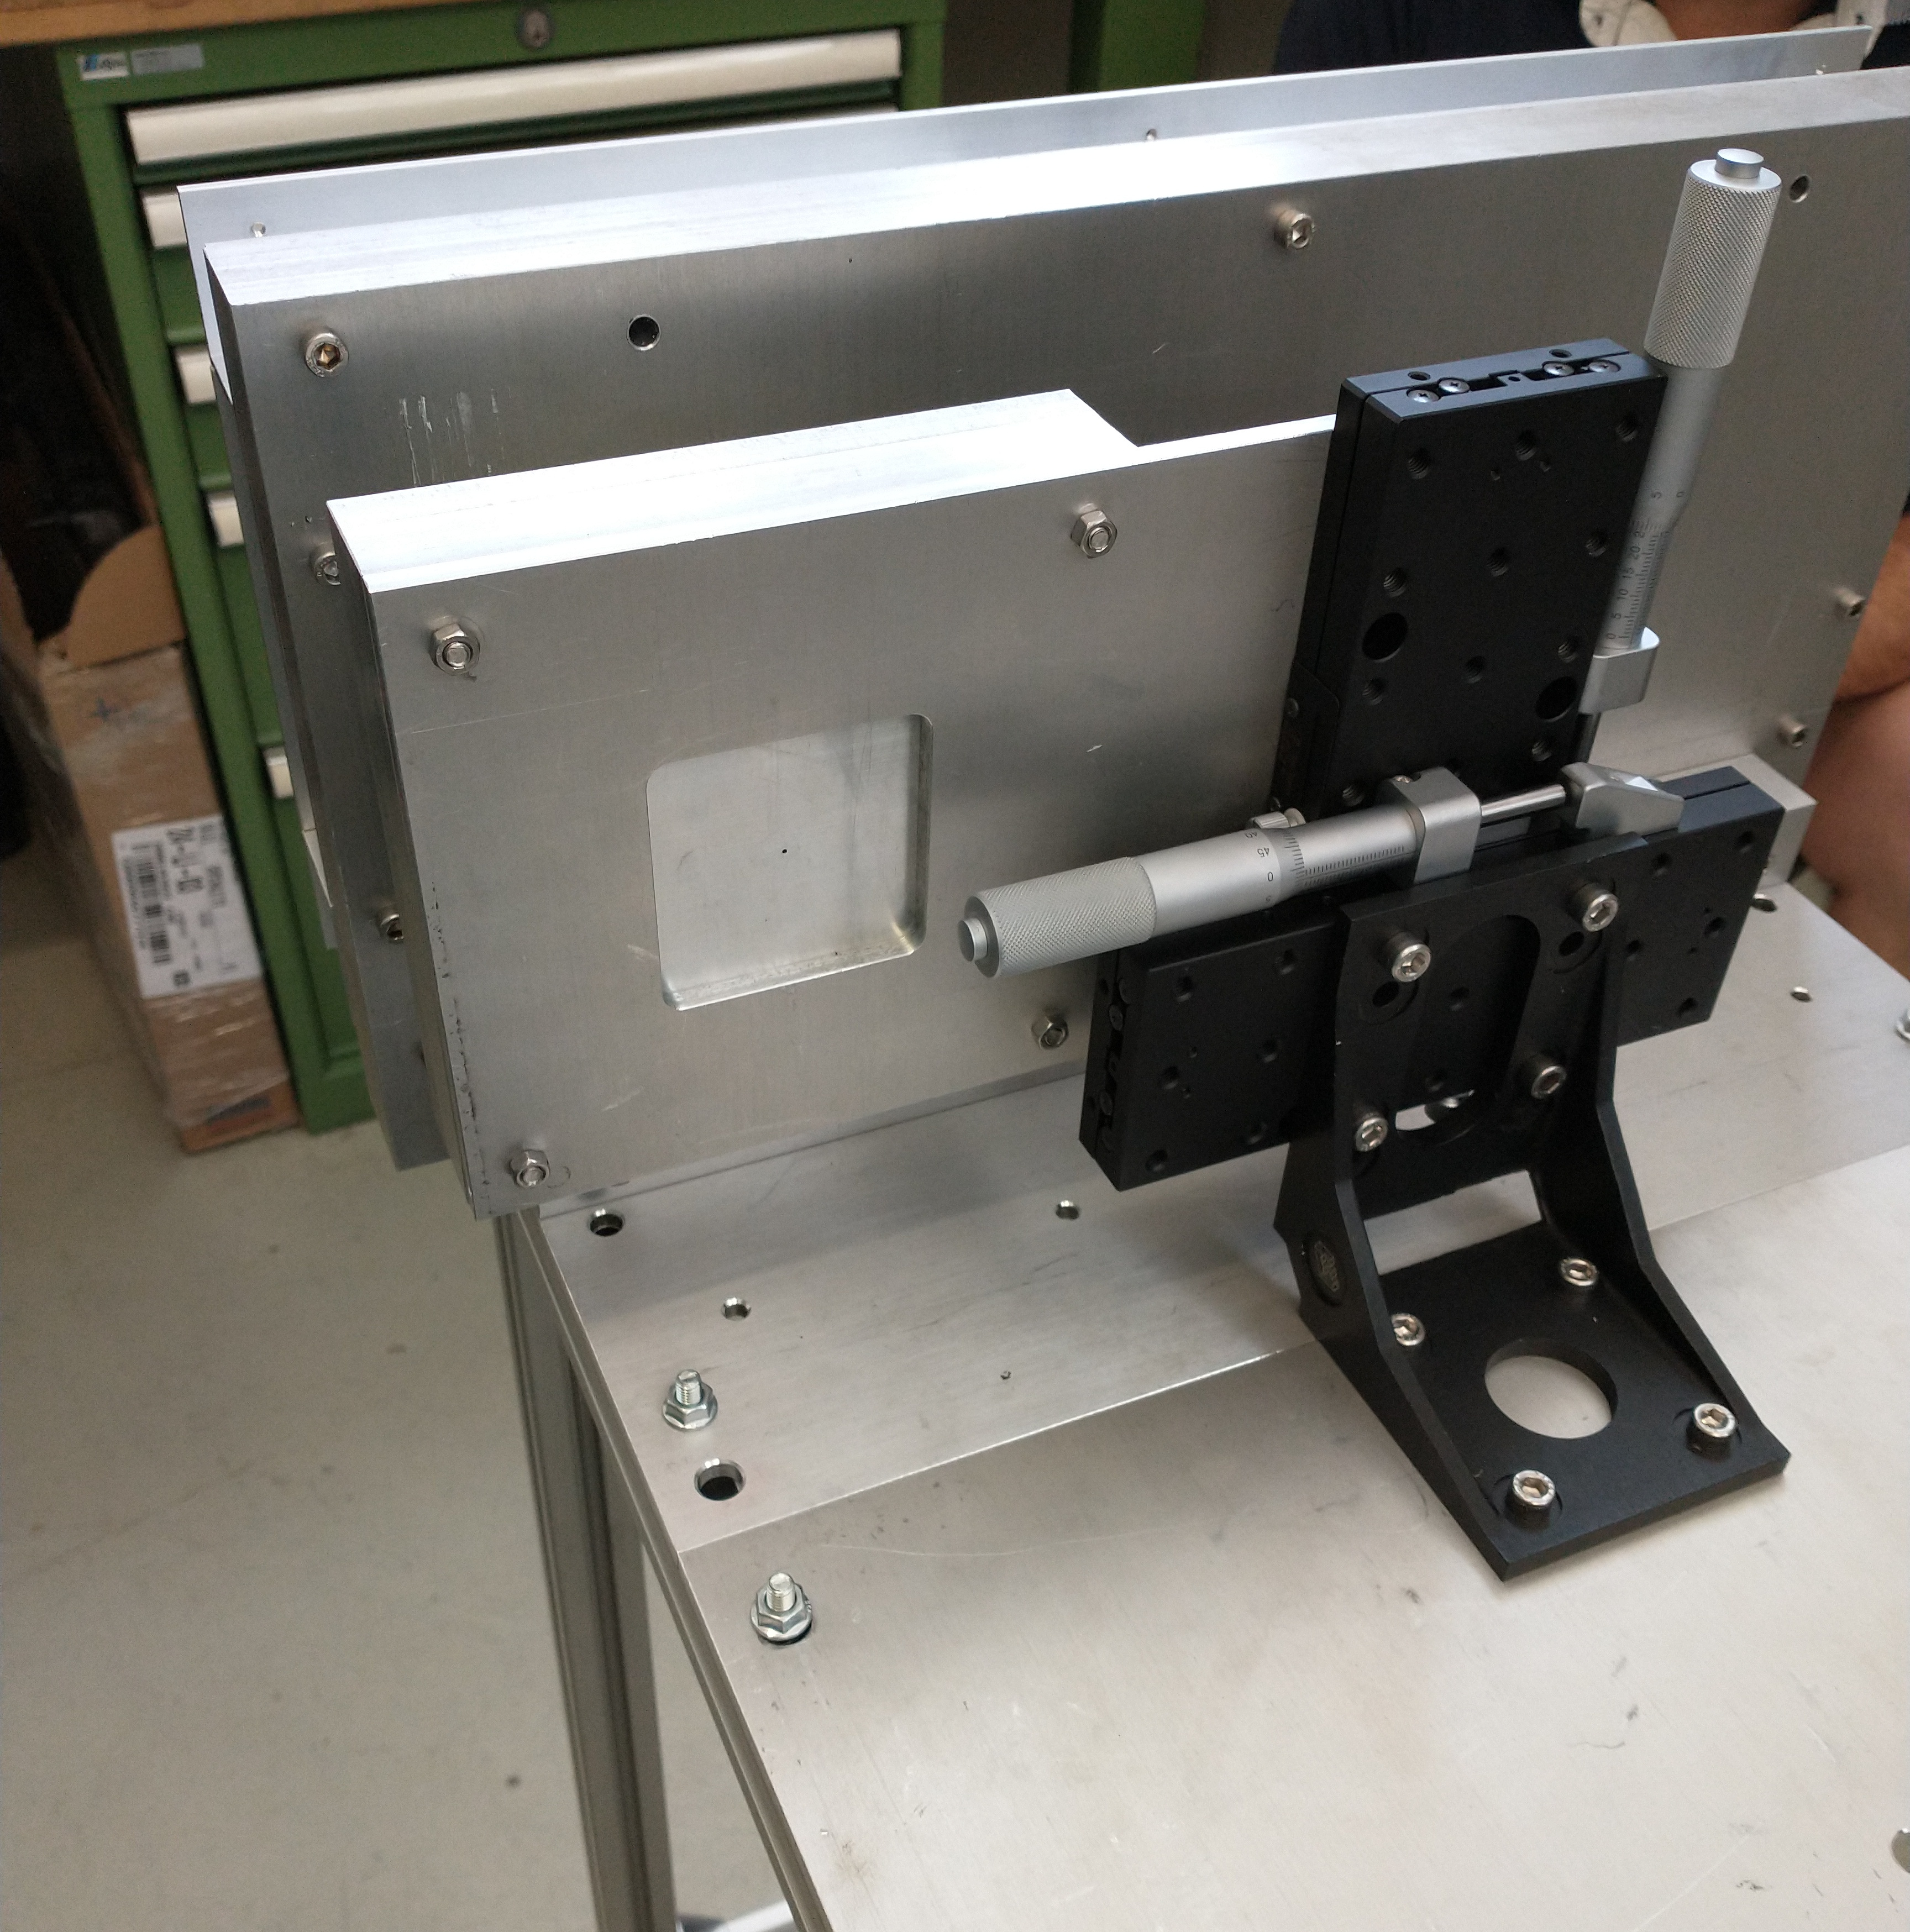
\includegraphics[width=.35\linewidth]{figures/test_beam/collimator_box.jpg}\\     
         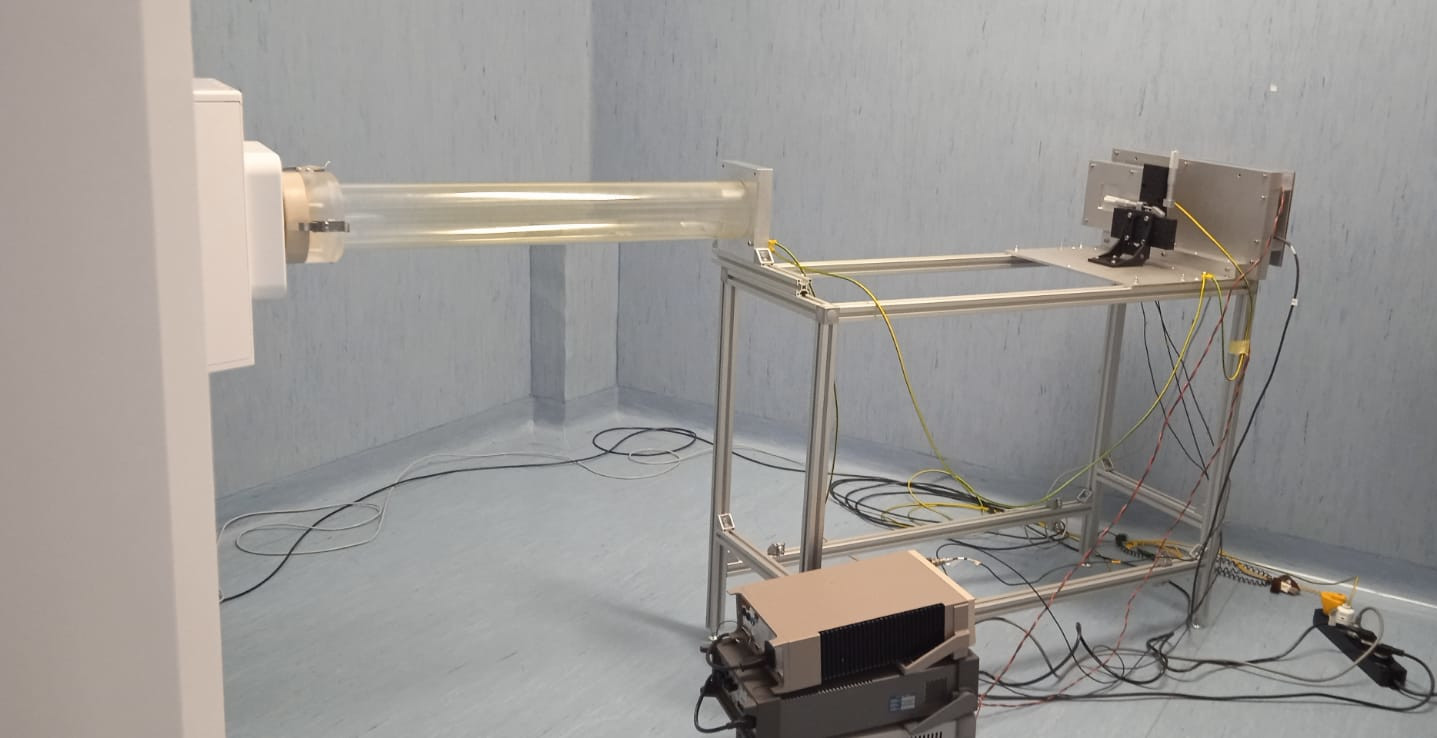
\includegraphics[width=.77\linewidth]{figures/test_beam/carrello.jpeg} 
         \label{fig:set_up}
         \caption{Experimental set up. (a) Electron flash accelerator: 
         gantry rotante che consente un orientamento del fascio da 0°
90° (orizzontale /verticale) in tempo reale monitorato da un inclinometro integrato.
         the gun can be rotated from \SI{90}{\degree} to \SI{0}{\degree} (vertical/orizontal). (b) Collimator and DUT box. (c) Whole structure: we used the \SI{10}{cm} diameter and \SI{1.2}{m} long triode; the DUT which is in the box behind the two collimators is connected to the power supply units.}
      \end{figure}  

\section{Measurements}
   Because of the dead time of TJ-Monopix1 it is not possible resolving the bunch sub-structure and almost no one pixel can read more than a hit per bunch. I recall, indeed, that the dead time per pixel depends on the location on the priority chain for the readout and for each pixel $\lesssim$\SI{1}{\us} (fig. \ref{fig:}) are needed; therefore only a few pixels at the top of the priority chain (at the upper left of the matrix) can fire a second time, since they in principle can be read the first time before the end of the pulse (assuming a pulse duration in \SI{2}{\us}-\SI{4}{\us}) and then can be hit again.

   Since resolving the single electron track is impossible, a way this sensor could be used in such context is reducing its efficiency and taking advantage of the analog pile up and of the linearity of the analog output (ToT), in order to see a signal produced not by the single particle but by more electrons. 
   Reducing the efficiency and the sensibility of the sensor is essential in order to decrease the high charge signal produced in the epitaxial layer: if the sensor is completely depleted the collection efficiency is closer to 1\% and if the whole charges produced by a MIP, \SI{80}{e-/\um} about, are collected, the saturation limit is soon reach. Then a condition where there is a partial recombination of the center electron-hole created in the bulk is desiderable.
   On the other hand, the smaller the output signal value and the higher the rate the detector can cope with: indeed, the rollover constitutes a limit for the usage of the analog output. 
   With the standard configuration of the FE parameters and the epitaxial layer completely depleted, a MIP produces a ToT out of range of representation of 6-bit; 
   so as to obtain smaller output signals one can operate on the reduction of the gain of the preamplifier or on the pulse velocity of returnig to the baseline. 
   Recalling the results in section \ref{chap:characterization_section:bias}, I have shown that concerning the PMOS flavor 1, reducing the bias from -\SI{6}{V} to \SI{0}{V} brings a reduction of efficiency down to \SI{40}{\%}, and a reduction in the gain of a factor $\sim$1/3, while the reduction of the gain of the preamplifier allows a reduction of \red{circa 10, ma da controllare}.
   
   In order to taking advantage of the analog pile up and integrating the charge, for semplicity assume of two electrons, the second one must hit the pixel before the ToT goes under the threshold. The general condition is then $\overline{\Delta T}<\overline{ToT}$, but if a high P$_\mu$($n\geqslant$1) is required, a lower $\overline{\Delta T}$ may be desired:
   \begin{equation}
      P(n\geqslant1) = \sum\limits_{n=1}^n \frac{e^{-\mu\;\mu^n}}{n!} = 1\;-\;P(0) = 1\;-\;e^{-\mu}
   \end{equation}
   \begin{equation}
      \mu = \frac{\overline{ToT}}{\overline{\Delta T}}
   \end{equation}
   If a P$_\mu$($n\geqslant$1) = 99\% then the $\overline{\Delta T}$ must be $\sim$0.22$\overline{ToT}$. The ToT is in range [0,64] but since the rollover must be avoided, the $\overline{ToT}$ must be lower than 32, and then the minimum rate on the pixel must be \SI{1.25}{\MHz}. \\   

   During the testbeam many runs have been performed, spanning the energy, the dose per pulse and the four possible configurations with/without the collimators. 
   We have used the PMOS flavor 1 in the standard configuration: we have biased the PWELL and PSUB at -\SI{6}{V} and set the standard default FE parameters reported in table \ref{tab:FE_default}.
   During all the acquisitions we have used pulses with t$_p$ of \SI{4}{\um} and with the smallest PRF settable, which is \SI{1}{Hz}, in order to start in the most conservative working point exluding the digital pile up of events from different bunch: even if the whole matrix turns on and there are 25000 hits, the total readout time corresponding to \SI{25}{ms} is still lower than the time between two consecutive pulses.
   The readout starts with the trailing edge of the first pulse going down the threshold, $\sim$\SI{50}{clk}=\SI{1.25}{\us} after this moment the FREEZE signal is sent to the whole matrix, and the trasmittion of the data to the EoC begins.
   The hits read are the ones whose TE occurred during the \SI{50}{clk} counts; the ones, instead, whose TE occur during the FREEZE are stored in the pixel memory and read during a second readout. Obviously since the readout of the fist sub-pulse finishes much later than the bunch ends up, each pixel can be store only one hit.   
   An example of the two sub-pulses is shown in figure \ref{fig:with collimator}: in the acquisition we injected 5 pulses with both the collimators mounted on the table. Looking at the spectrum \red{si vede che lo spettro del secondo pulse ha una coda più lunga a destra: questo è dovuto al fatto che le hit con tot lungo hanno il TE che cade durante il FREEZE e quindi vengono lette durante il secondo impulso}. On the other hand the 2D histograms, being uniform and not showing disomogenities, suggest that the collimators do not shield all the particles: this was due to a photon background higher than expected. 
   \red{When we have put aside the collimators, instead, the fluence was too high that the whole matrix turns on in \SI{50}{clk} counts; then the 2 pulses substructure no more appears (fig. \ref{fig:without_collimator}).  CONTROLLA PERCHÈ PORTEBBE ESSERE UNA CAZZATA}
   \begin{figure}
      \centering
      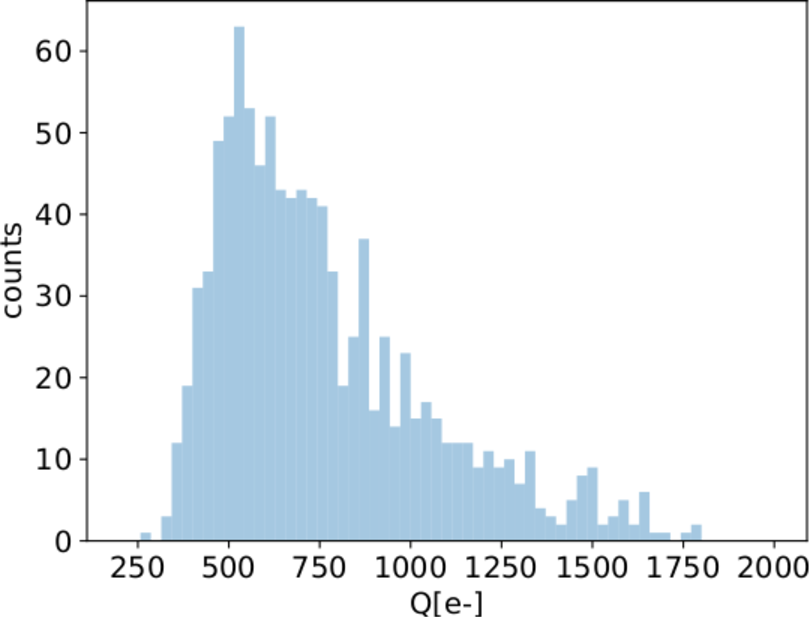
\includegraphics[width=.49\linewidth]{figures/test_beam/Q1_17_11.pdf}
      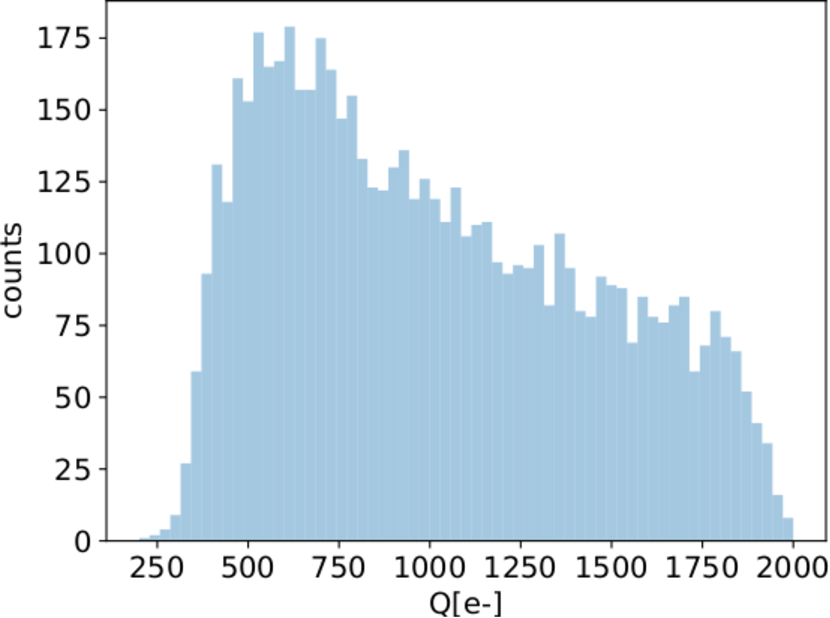
\includegraphics[width=.49\linewidth]{figures/test_beam/Q2_17_11.pdf}\\   
      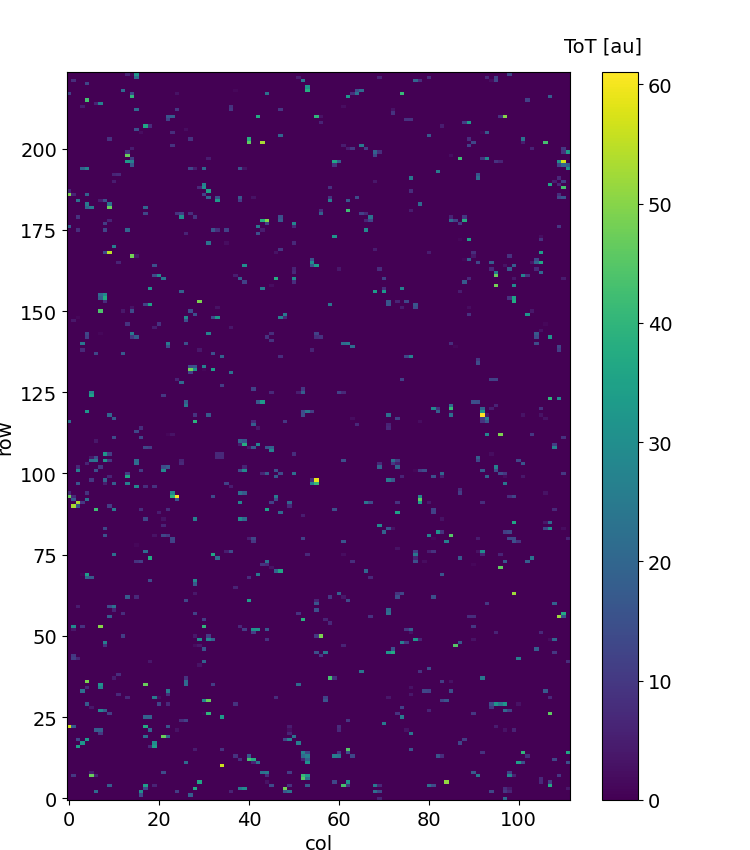
\includegraphics[width=.49\linewidth]{figures/test_beam/tot_mapq1_17-11.png}
      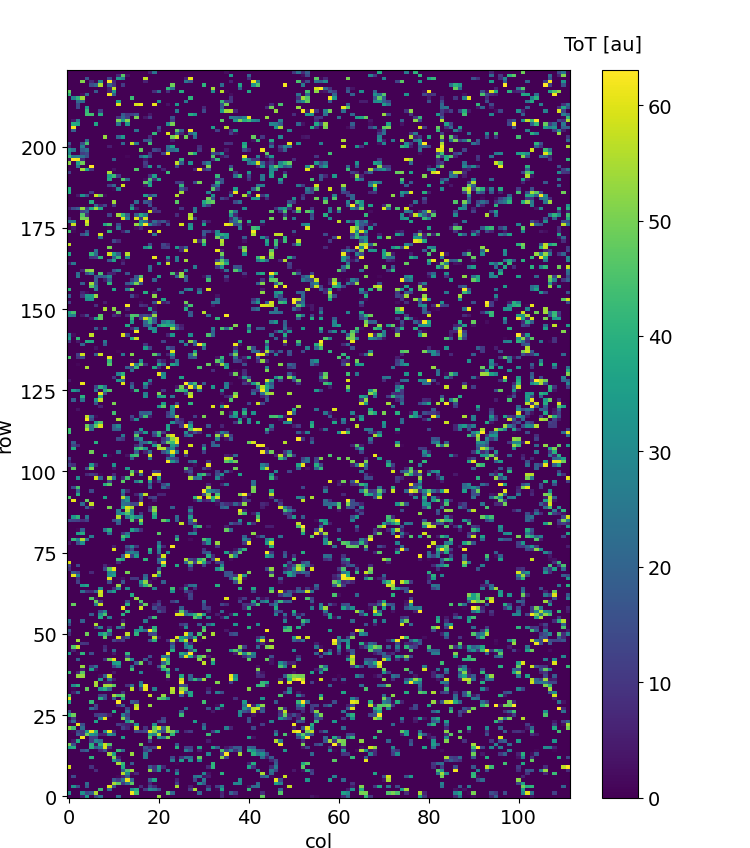
\includegraphics[width=.49\linewidth]{figures/test_beam/tot_mapq2_17-11.png} 
      \caption{Acquisition with both the collimators: 5 pulses at DDP=\SI{0.07}{Gy}. (a) Spectrum of the charge released in the sensor: to apply the conversion I used the information found in the previous chapter. (b) 2D histogram of the ToT of the hits arrived in the sub-pulses. }
      \label{fig:with_collimator}
   \end{figure}
   \begin{figure}
      \centering
      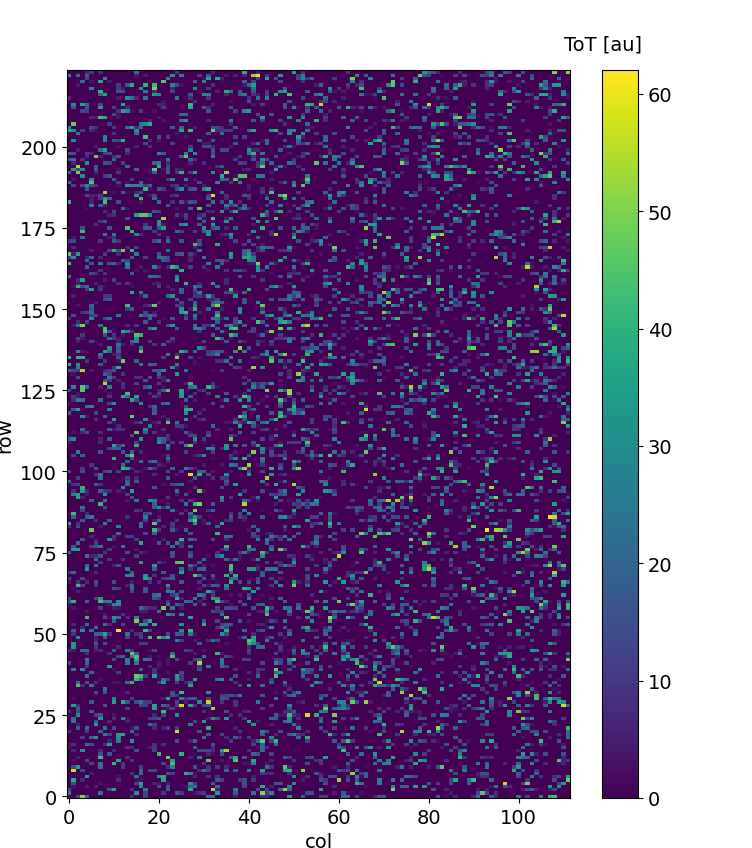
\includegraphics[width=.49\linewidth]{figures/test_beam/tot_mapq1_15-57.png}
      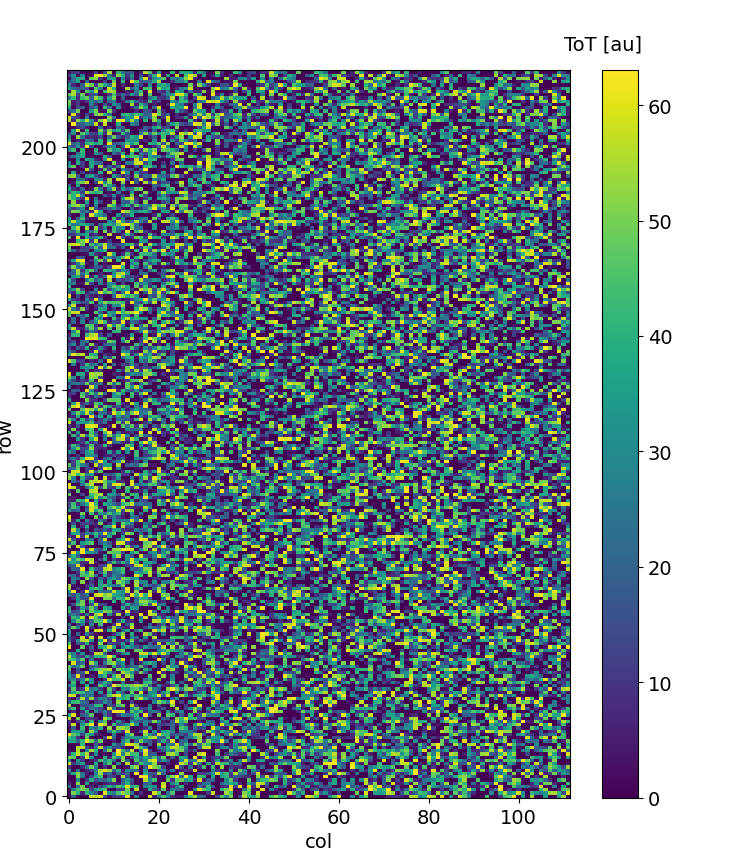
\includegraphics[width=.49\linewidth]{figures/test_beam/tot_mapq2_15-57.png}  
      \caption{Acquisition with both the collimators: 5 pulses at DDP=\SI{0.6}{Gy}. 2D histogram of the ToT of the hits arrived in the sub-pulses. Compared with the previous maps, since the DDP is much higher, more pixels turn on.}
      \label{fig:}
   \end{figure}
   \begin{figure}
      \centering
      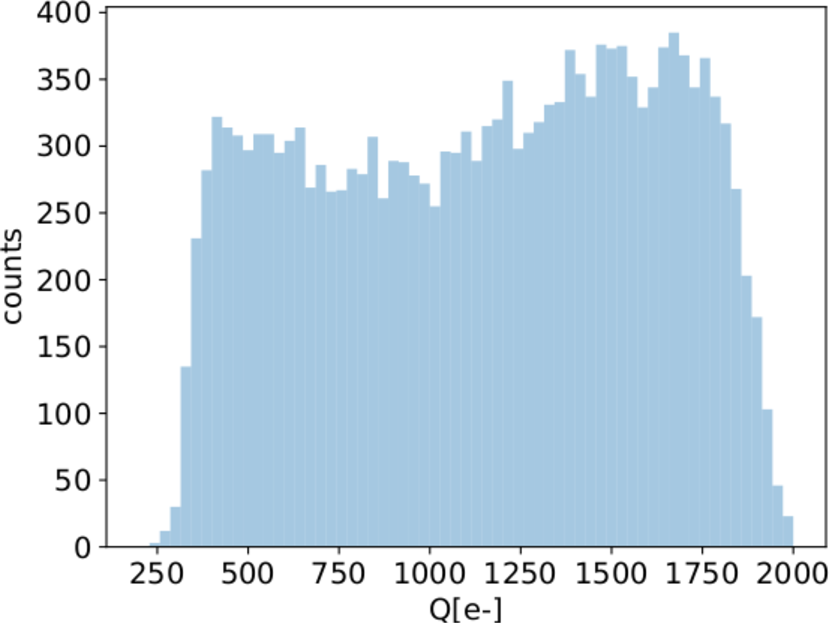
\includegraphics[width=.7\linewidth]{figures/test_beam/Qe_17_32.pdf}
      \caption{Acquisition without any collimator: 5 pulses at DDP=\SI{0.04}{Gy}.}
      \label{fig:without_collimator}
   \end{figure}

   After the testbeam a simulation of the emission of electrons from the accelerator and their path across the triode and the collimators has been developed via Geant-4 \red{come si ringrazia il lavoro di qualcuno in maniera formale?}. 
   The high background we saw although the collimators were mainly produced by electrons Bremsstrahlung during the transition through the alluminium collimators. \red{dalla simulazione si è visto che nessun elettrone arriva sul chip quando ci sono montati i collimatori, mentre nel caso senza collimatori gli eventi sono sostanzialmente tutti elettroni (frazione di fotoni prodotti in aria è?).}
   The photons' simulated spectrum in the three configurations are shown in figure \ref{fig:MC_photons_spectrum}. \red{confronto con quello che vedo nello spettro sopra: dati.}
   \red{
   \begin{itemize}
      \item plot n di eventi che vedo con le diverse configurazioni
      \item simulazione surya
      \item confronta con misure dello spettro che vediamo senza e con collimatori. 
   \end{itemize}
   }

   \subsection{MIP spectrum using cosmic rays as source}
      Since a MIP should produce about \SI{2}{ke-} in the epitaxial layer, it should provide a signal that in our conditions (full depletion and high gain) rolls over: in this situation making prediction on the spectrum expected for MIPs becomes hard. 
      Therefore, in order to compare the spectrum observed at the testbeam with one certainly produced by MIP I have made some acquisitions without any radioactive source, in order to look at the cosmic ray events. 
      To be confident with having selected MIPs from cosmic rays and cut the noise, I have selected only the events with multiple hits: these events are mainly clusters produced by the same impinging particle since the random coincidence probability is very low. 
      In fact the cosmic rays and noise rates on the whole matrix are respectively \SI{0.02}{Hz} and $\sim$\si{Hz}, the dead time in such a low occupancy condition can be alway approximated with \SI{1}{\um} (this is not completely true for multiple hits events for which the the priority chain should be considered), the random coincidence rate is 10$^{-8}$\si{Hz}.
       \begin{figure}
          \centering
          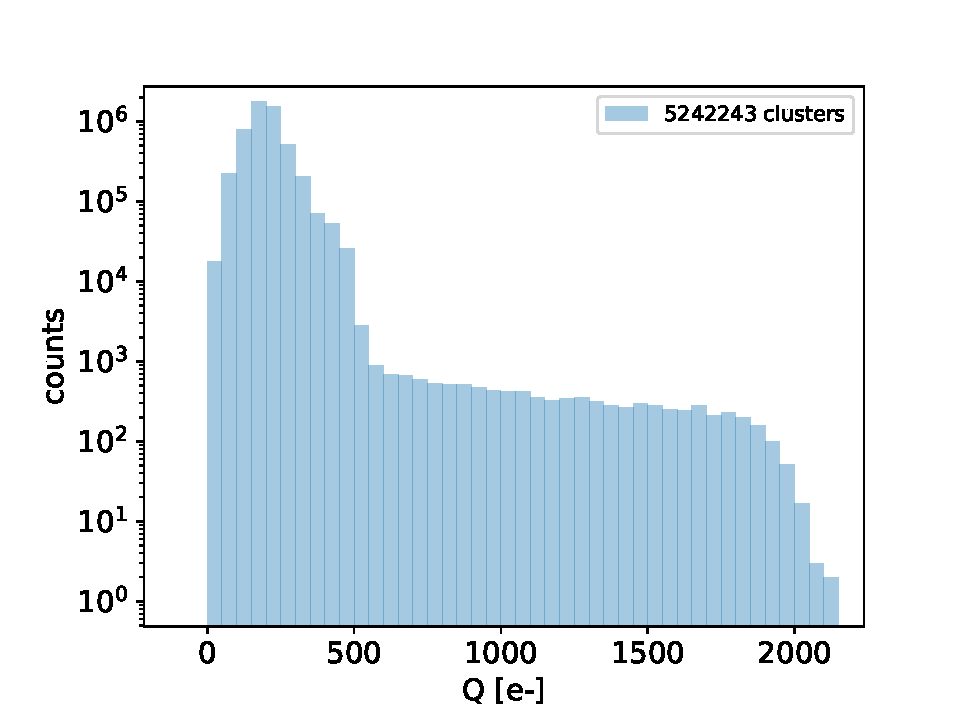
\includegraphics[width=.49\linewidth]{figures/test_beam/MIP/all_evts.pdf}
          \includegraphics[width=.49\linewidth]{figures/test_beam/MIP/only_evts_with_cluster.pdf}\\   
          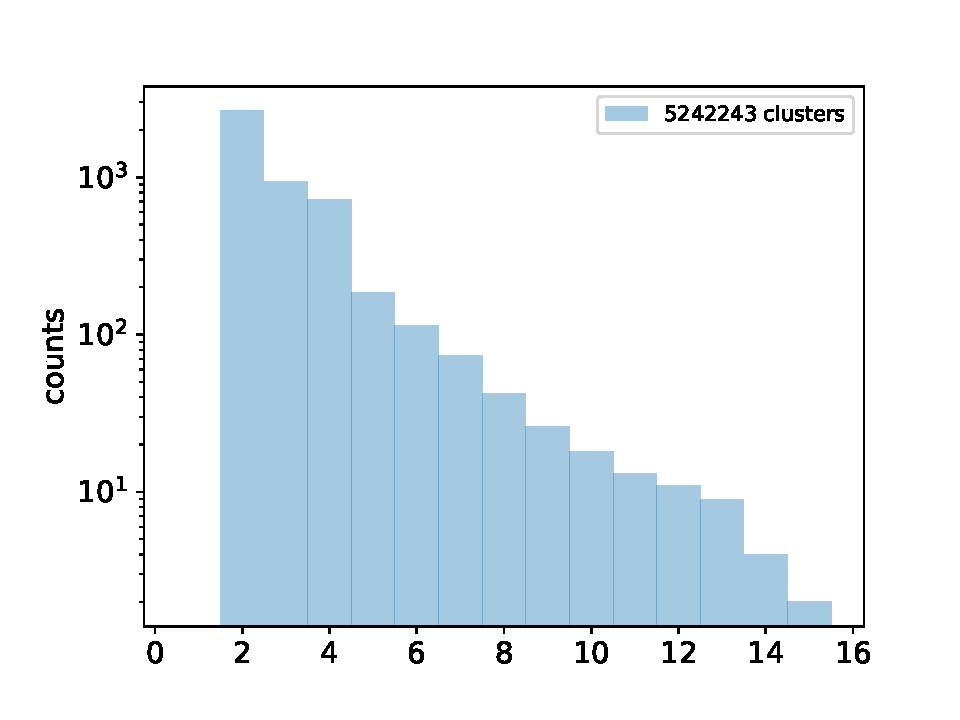
\includegraphics[width=.49\linewidth]{figures/test_beam/MIP/hits_per_cluster.pdf}
          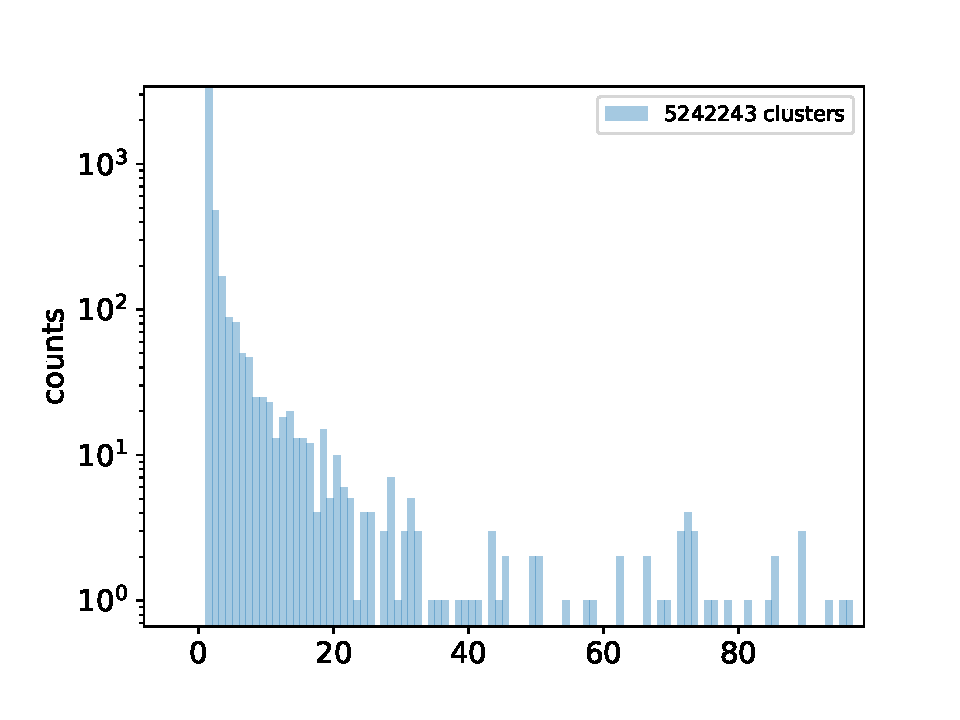
\includegraphics[width=.49\linewidth]{figures/test_beam/MIP/cluster_dimension.pdf} 
          \caption{\red{plot dei raggi cosmici da rigenerare}}
          \label{fig:}
       \end{figure}   
       \red{Come mai lo spettro in lab è diverso da quello visto con gli elettroni da 9 MeV al santa chiara? Chiedi a Surya il rate visto sul detector senza collimatori. }
   

